%%%%%%%%%%%%%%%%%%%%%%%%%%%%%%%%%%%%%%%%%
% Beamer Presentation
% LaTeX Template
% Version 1.0 (10/11/12)
%
% This template has been downloaded from:
% http://www.LaTeXTemplates.com
%
% License:
% CC BY-NC-SA 3.0 (http://creativecommons.org/licenses/by-nc-sa/3.0/)
%
%%%%%%%%%%%%%%%%%%%%%%%%%%%%%%%%%%%%%%%%%

%----------------------------------------------------------------------------------------
%	PACKAGES AND THEMES
%----------------------------------------------------------------------------------------

%\documentclass{beamer}
\documentclass[12pt, aspectratio=169]{beamer}
\usepackage{keynote-gradient-white}

\mode<presentation> {

% The Beamer class comes with a number of default slide themes
% which change the colors and layouts of slides. Below this is a list
% of all the themes, uncomment each in turn to see what they look like.

%\usetheme{default}
%\usetheme{AnnArbor}
%\usetheme{Antibes}
%\usetheme{Bergen}
%\usetheme{Berkeley}
%\usetheme{Berlin}
%\usetheme{Boadilla}
%\usetheme{CambridgeUS}
%\usetheme{Copenhagen}
%\usetheme{Darmstadt}
%\usetheme{Dresden}
%\usetheme{Frankfurt}
%\usetheme{Goettingen}
%\usetheme{Hannover}
%\usetheme{Ilmenau}
%\usetheme{JuanLesPins}
%\usetheme{Luebeck}
%\usetheme{Madrid}
%\usetheme{Malmoe}
%\usetheme{Marburg}
%\usetheme{Montpellier}
%\usetheme{PaloAlto}
%\usetheme{Pittsburgh}
%\usetheme{Rochester}
%\usetheme{Singapore}
%\usetheme{Szeged}
%\usetheme{Warsaw}

% As well as themes, the Beamer class has a number of color themes
% for any slide theme. Uncomment each of these in turn to see how it
% changes the colors of your current slide theme.

%\usecolortheme{albatross}
%\usecolortheme{beaver}
%\usecolortheme{beetle}
%\usecolortheme{crane}
%\usecolortheme{dolphin}
%\usecolortheme{dove}
%\usecolortheme{fly}
%\usecolortheme{lily}
%\usecolortheme{orchid}
%\usecolortheme{rose}
%\usecolortheme{seagull}
%\usecolortheme{seahorse}
%\usecolortheme{whale}
%\usecolortheme{wolverine}

%\setbeamertemplate{footline} % To remove the footer line in all slides uncomment this line
%\setbeamertemplate{footline}[page number] % To replace the footer line in all slides with a simple slide count uncomment this line

%\setbeamertemplate{navigation symbols}{} % To remove the navigation symbols from the bottom of all slides uncomment this line
}

\usepackage{graphicx} % Allows including images
\usepackage{booktabs} % Allows the use of \toprule, \midrule and \bottomrule in tables
\usepackage{hyperref}

\setbeamertemplate{footline}[frame number]

%--------------------------------------------------------------------------------
%	TITLE PAGE
%--------------------------------------------------------------------------------

\title[Neurointerface implemented with Oscillator Motifs]{Neurointerface implemented with Oscillator Motifs} % The short title appears at the bottom of every slide, the full title is only on the title page

\author[Max Talanov]{
  Max Talanov$^{1,2}$, Alina Suleimanova$^{1,2}$, Alexey Leukhin$^{1,2}$,
  Yulia Mikhailova$^{1,2}$, Alexander Toschev$^{1,2}$,
  Alena Militskova$^{3}$, Igor Lavrov$^{1,5}$, Evgeni Magid$^{4}$
}

% Alina Suleimanova$^{1,2}$, Alexey Leukhin$^{1,2}$,Yulia Mikhailova$^{1,2}$, Alexander Toschev$^{1,2}$, \\ Alena Militskova$^{3}$, Igor Lavrov$^{1,5}$, Evgeni Magid$^{4}$

\institute[B-Rain Labs LLC, NcN laboratory, ITIS, KFU]% Your institution as it will appear on the bottom of every slide, may be shorthand to save space
{
  $^{1}$ B-Rain Labs LLC;
  $^{2}$ Neuromorphic computing and Neurosimulations laboratory, ITIS, KFU;
  $^{3}$ Institute of Fundamental Medicine and Biology, KFU;
  $^{4}$ Intelligent Robotic Systems Laboratory (LIRS), ITIS, KFU;
  $^{5}$ Department of Neurologic Surgery, Department of Physiology and Biomedical Engineering, Department of Neurology at Mayo Clinic.
  
  % Your institution for the title page
\medskip
\textit{max.talanov@b-rain.org}\\ % Your email address

}
\date{IROS-2021} % Date, can be changed to a custom date

\begin{document}

\begin{frame}
\titlepage % Print the title page as the first slide
\end{frame}


%-------------------------------------------------------------------------------
% Kevin Warwick
%-------------------------------------------------------------------------------

%------------------------------------------------
\section{Kevin Warwick}
%------------------------------------------------
\begin{frame}
  \frametitle{Kevin Warwick fist cyborg}
  \begin{figure}
    \includegraphics[width=0.7\linewidth]{Kevin-Warwick_2936650k}
  \end{figure}
  \footnotetext{\url{https://www.telegraph.co.uk/}}
\end{frame}

%-------------------------------------------------------------------------------
% Neuralink
%-------------------------------------------------------------------------------

%------------------------------------------------
\section{Neuralink}

%------------------------------------------------
\begin{frame}
  \frametitle{Neuralink: link interface}
  \begin{figure}
    \includegraphics[width=0.4\linewidth]{approach-link-1}
  \end{figure}
  \footnotetext{https://neuralink.com/approach/}
\end{frame}

%------------------------------------------------

%-------------------------------------------------------------------------------
% Neurointeface architecture
%-------------------------------------------------------------------------------

%------------------------------------------------
\section{Architecture}
%------------------------------------------------
\begin{frame}
  \frametitle{Neurointerface architecture}
  \begin{figure}
    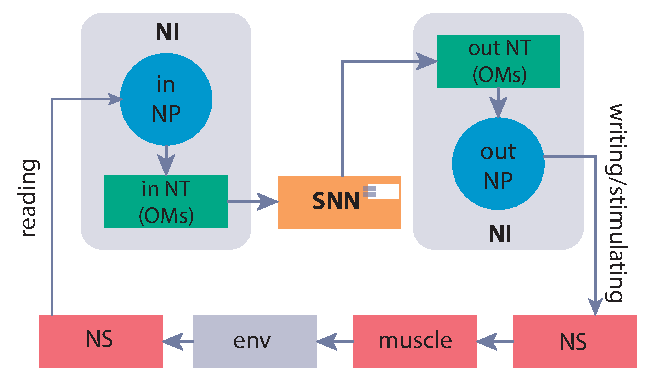
\includegraphics[width=0.9\linewidth]{NI_h}
  \end{figure}
\end{frame}

%------------------------------------------------
\begin{frame}
  \frametitle{Experimental setup}
  \begin{figure}
    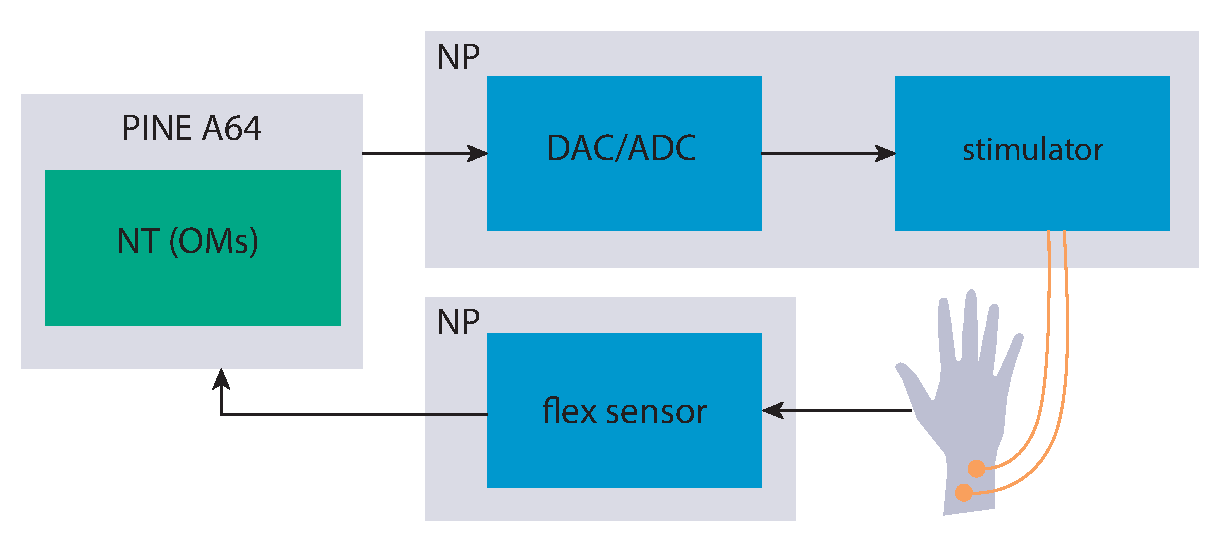
\includegraphics[width=0.9\linewidth]{hld_exp}
  \end{figure}
\end{frame}
%------------------------------------------------
\section{Oscillator motif}
%------------------------------------------------
\begin{frame}
  \frametitle{Oscillator motif}
  \begin{figure}
    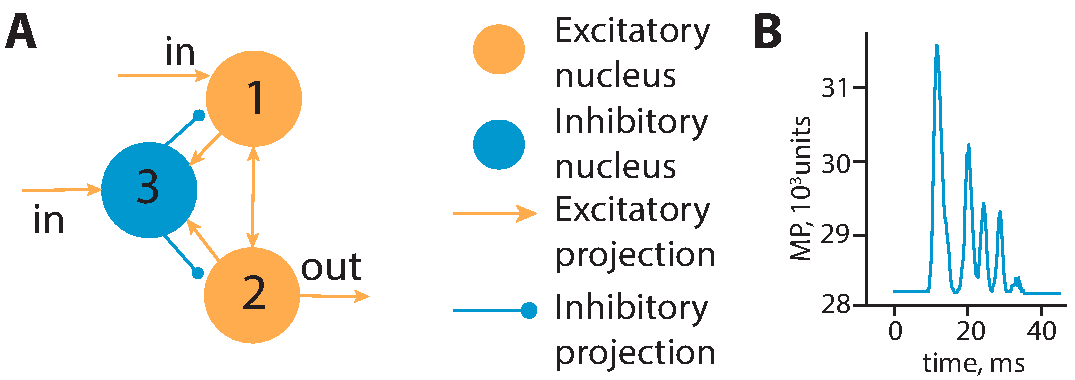
\includegraphics[width=0.8\linewidth]{OM_2}
  \end{figure}
\end{frame}
%------------------------------------------------
\begin{frame}
  \frametitle{Oscillator motif networks}
  \begin{figure}
    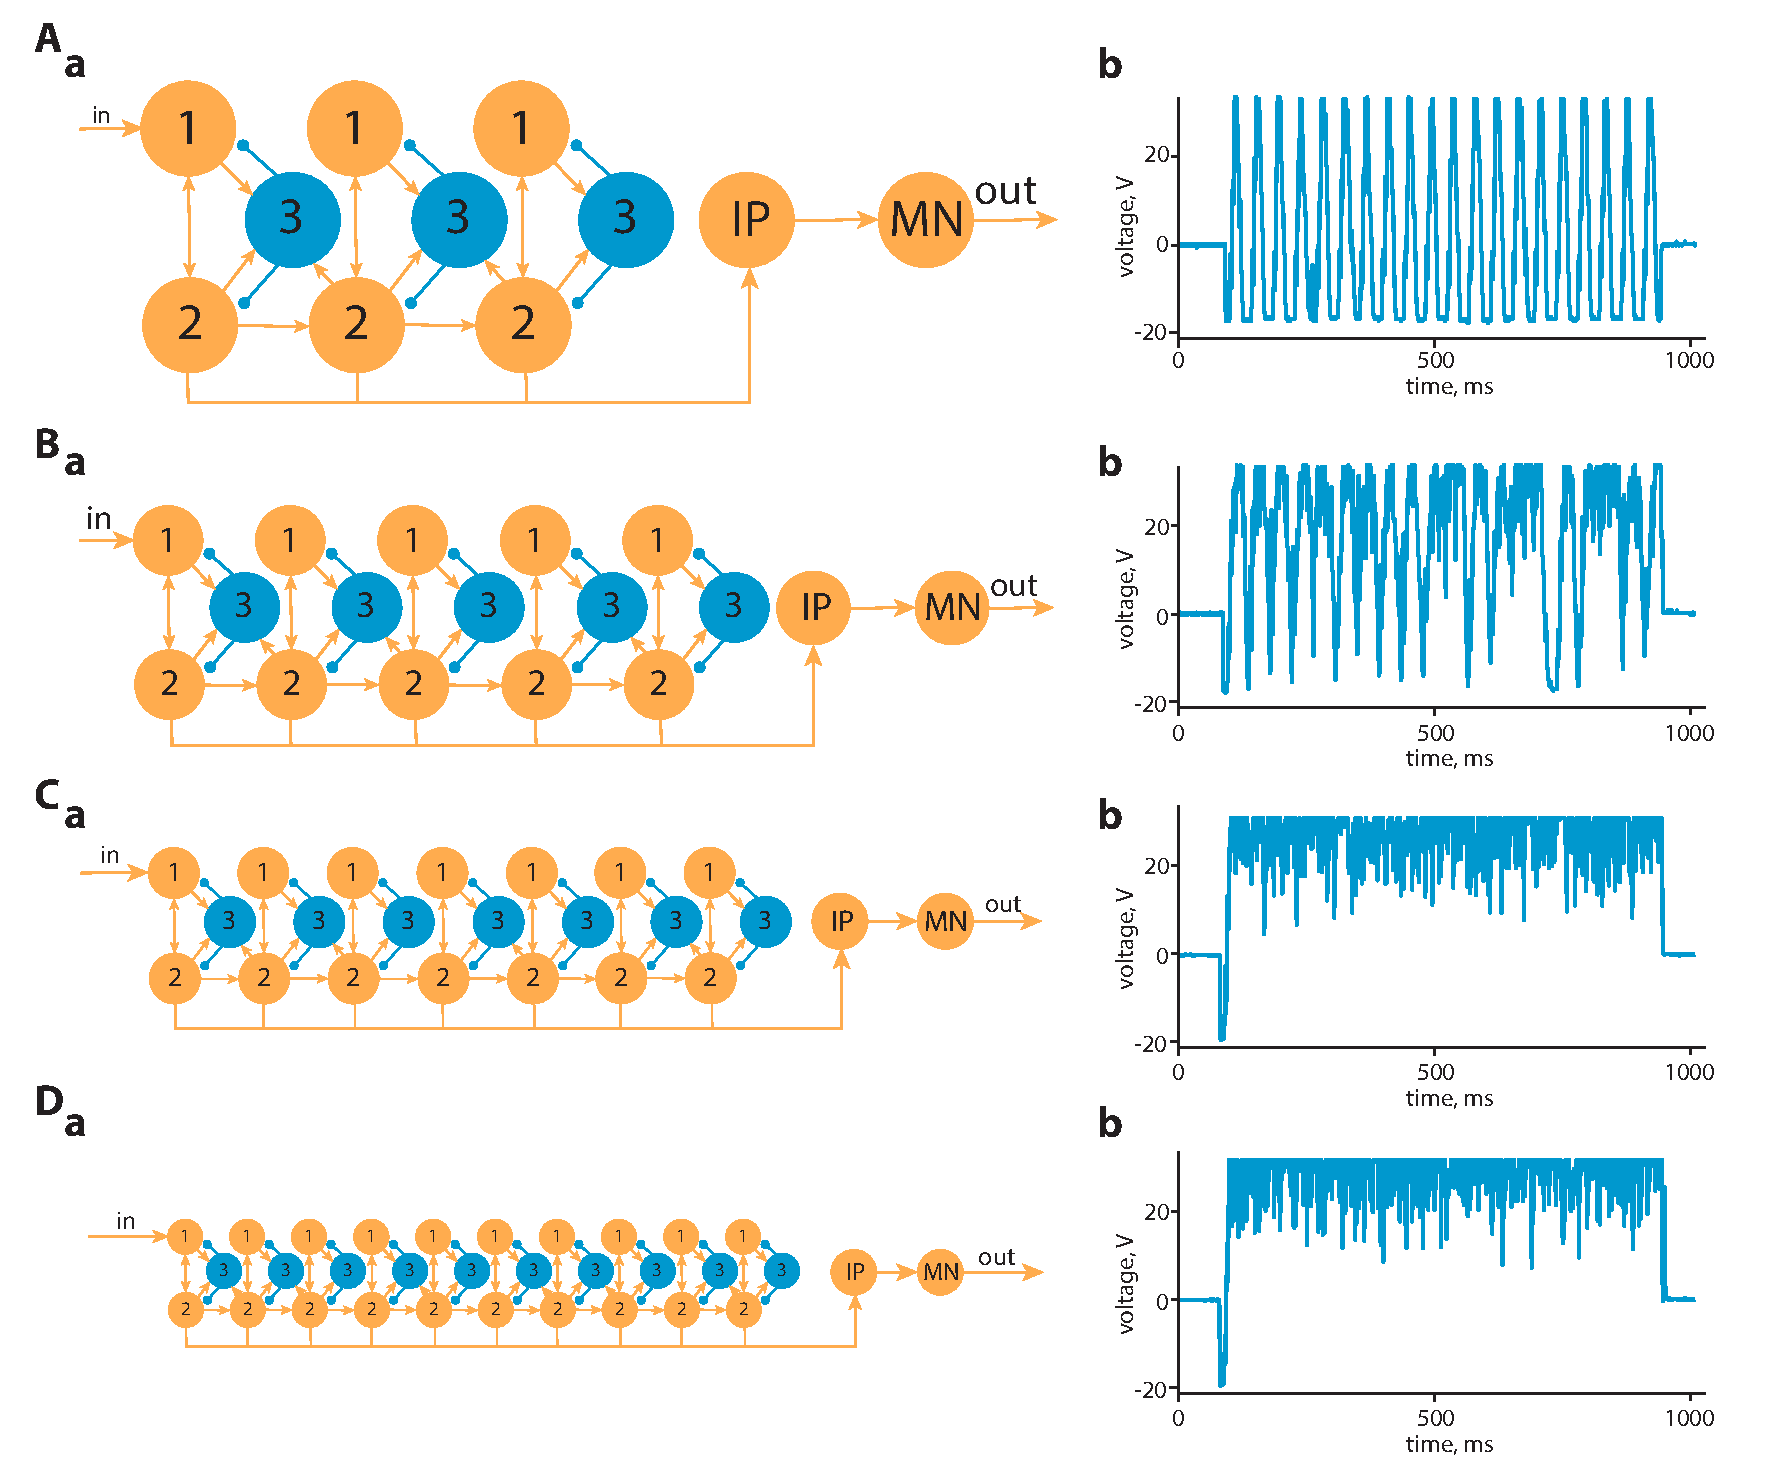
\includegraphics[width=0.65\linewidth]{OM_osc}
  \end{figure}
\end{frame}
%------------------------------------------------

%------------------------------------------------
\section{Results}
%------------------------------------------------
\begin{frame}
  \frametitle{Results: finger displacement}
  \begin{figure}
    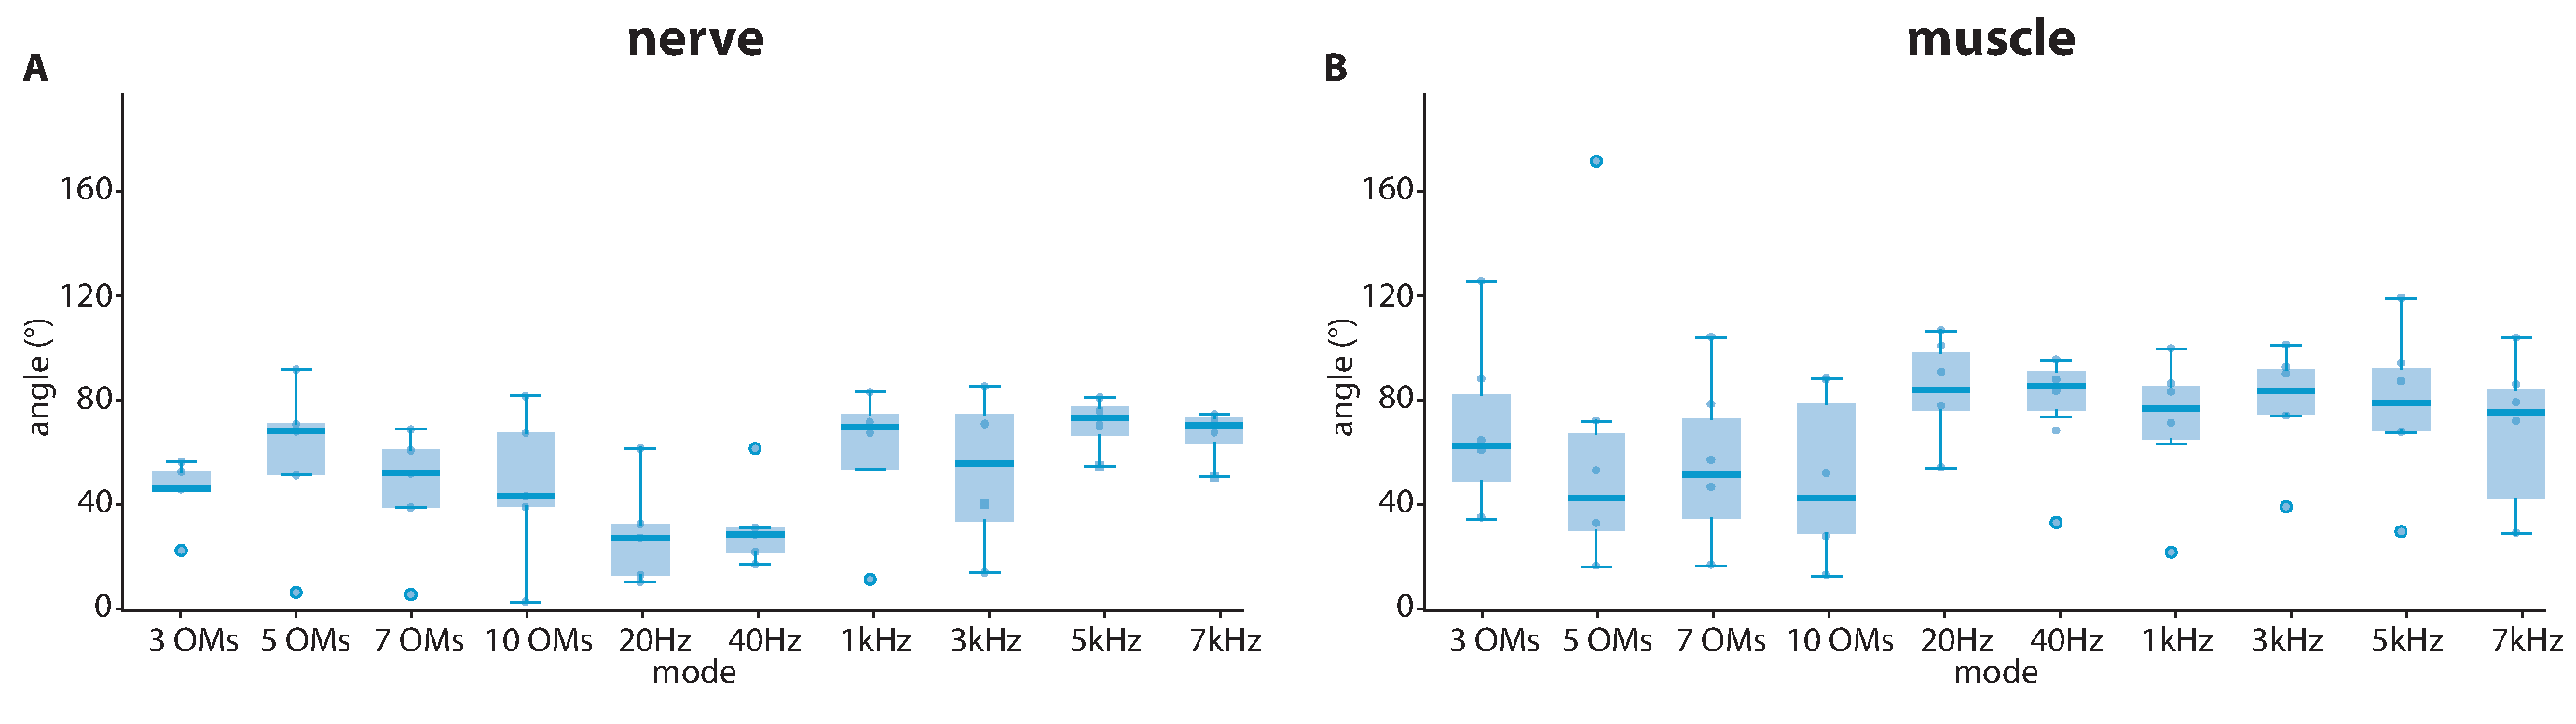
\includegraphics[width=1.0\linewidth]{angles_all}
  \end{figure}
\end{frame}
%------------------------------------------------
\begin{frame}
  \frametitle{Results: discomfort rate}
  \begin{figure}
    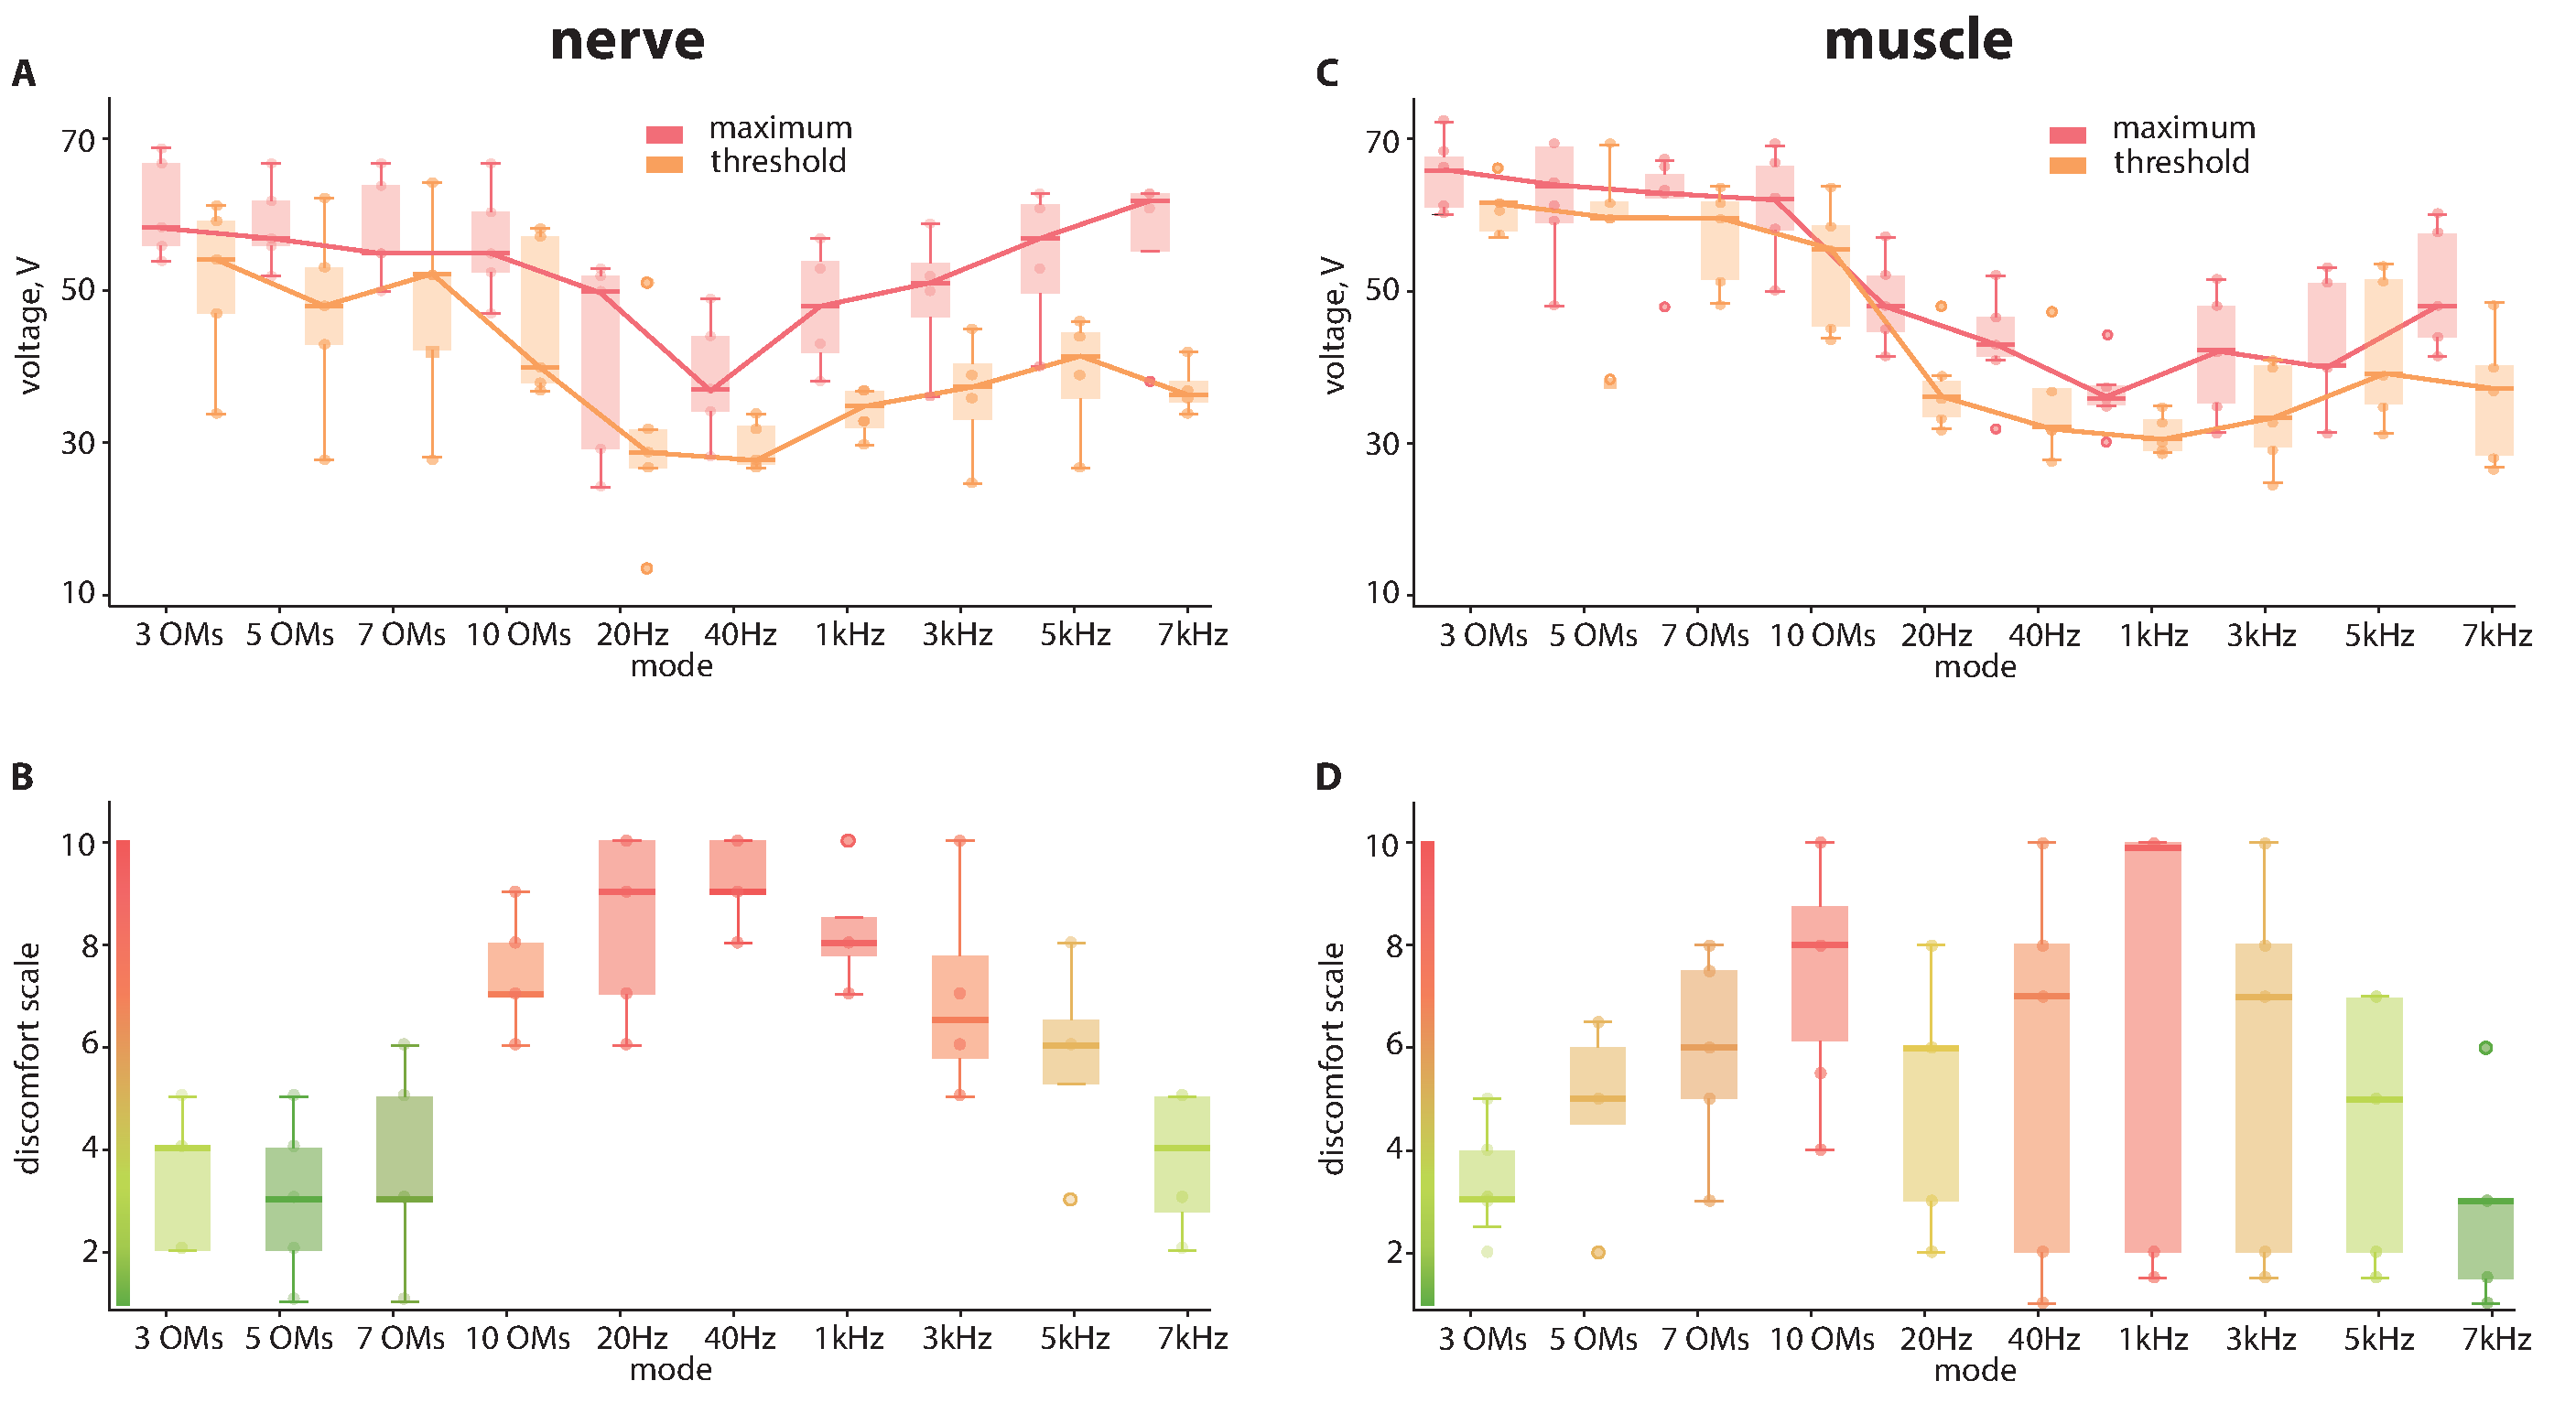
\includegraphics[width=0.9\linewidth]{threshold_angle}
  \end{figure}
\end{frame}
%------------------------------------------------
%Conclusion
%------------------------------------------------
\begin{frame}
  \frametitle{Conclusion}
\begin{columns}[c]
\column{.7\textwidth} % Left column and width
 
\begin{itemize}
  \item We proposed the neurosimulation based neurointerface architecture.
  \item We conducted experiments to identify the impact of neurosimulation over muscle and nerve stimulation.
  \item The most comfortable mode for the nerve stimulation was the 5~OMs 3.0/10, the maximum angle of finger displacement 57.4$^{\circ}$.
  \item The optimal modes for sensation and deflection angle are 5 and 7 OMs for nerve stimulation and 3 OMs for muscle stimulation.
\end{itemize}

\column{.3\textwidth} % Right column and width
\begin{figure}
\includegraphics[width=1.0\linewidth]{mousebrainpink}
\end{figure}
\end{columns}
\end{frame}
%------------------------------------------------
%------------------------------------------------
\begin{frame}
  \frametitle{Acknowledgment}
The authors would like to thank the B-Rain Labs LLC company for supporting their work with neurosimulations. The eighth author acknowledges the support of the Russian Foundation for Basic Research (RFBR), project ID 19-58-70002. 
This work is the part of Kazan Federal University Strategic Academic Leadership Program. 

\end{frame}
%------------------------------------------------
%------------------------------------------------
\begin{frame}
  \frametitle{Oscillator motif simulation}
  \begin{figure}
    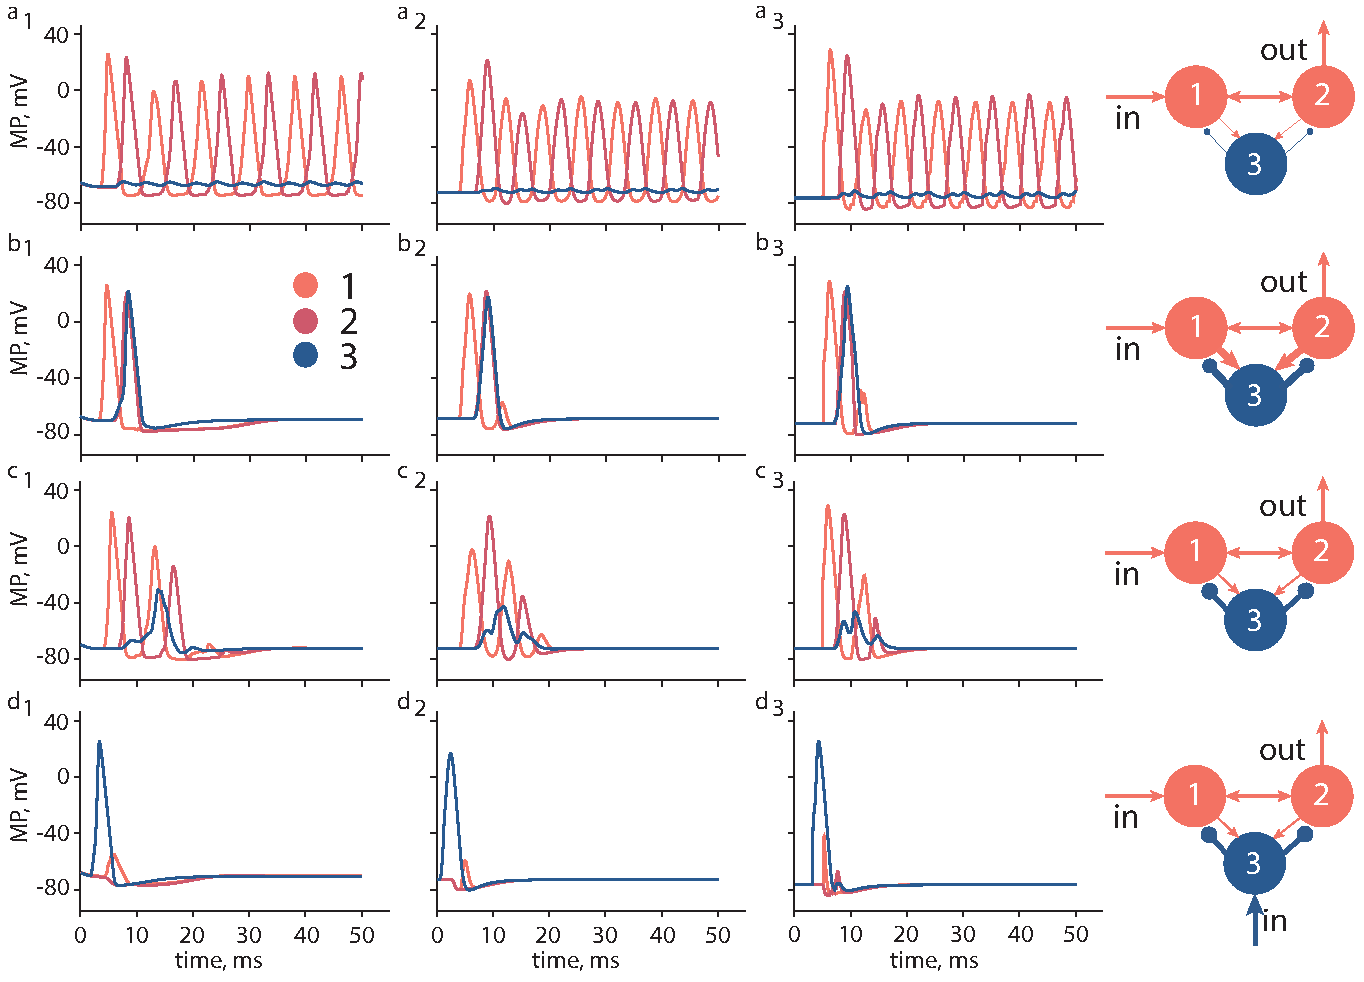
\includegraphics[width=0.7\linewidth]{OM_sim}
  \end{figure}
\end{frame}

%------------------------------------------------
\begin{frame}
  \frametitle{Future work}
\begin{columns}[c]
\column{.6\textwidth} % Left column and width

\textbf{Reflex arc:}\\
1754 neurons, 478 200 synapses,\\
Motor neuron - 400 synapses,\\
Ia interneuron - 300,
Ib interneuron - 200,\\
Renshaw - 200,
Afferents - 100\\

\textbf{Central pattern generator:}\\
880 interneurons including interneuronal pool,
40 000 synapses,
each nucleaus 20 neurons

\column{.4\textwidth} % Right column and width
\begin{figure}
\includegraphics[width=1.0\linewidth]{mousebrainpink}
\end{figure}
\end{columns}
\end{frame}

%------------------------------------------------

\end{document} 
